\section{Contrôle et suivi du projet}
\markboth{5. Contrôle et suivi du projet}{}

\subsection{Tableau de bord de pilotage}

\subsubsection*{Indicateurs suivis}

\begin{table}[H]
\centering
\small
\begin{tabularx}{\linewidth}{@{}L{2.5cm}L{4.6cm}XL{2.1cm}@{}}
\toprule
\textbf{Dimension} & \textbf{Indicateur} & \textbf{Valeur au terme du projet} & \textbf{Fréquence} \\
\midrule
Délais & Phases achevées & 6 sur 6 & Par phase \\
Coûts & Coût d'infrastructure récurrent & 0\,\$ & Mensuelle \\
Livrables & Application, dépôt, tests, rapport & Livrés & Par phase \\
\midrule
Qualité des données & Lignes retenues après nettoyage & \num{1655} sur \num{1656} & Par millésime \\
& Écarts documentés vis-à-vis de l'existant & 16 & Au fil de l'eau \\
& Modalités inconnues acceptées silencieusement & 0 (exception levée) & Continu \\
\midrule
Performance ML & $R^2$ hors bloc, énergie & 0,745 & Par réentraînement \\
& $R^2$ hors bloc, émissions & 0,723 & Par réentraînement \\
& Erreur relative médiane & 36,6\,\% / 45,1\,\% & Par réentraînement \\
& Couverture observée des fourchettes & 81,3\,\% / 81,0\,\% & Par réentraînement \\
\midrule
Qualité logicielle & Tests automatisés & 61, tous au vert & À chaque \emph{commit} \\
& Analyse statique & Sans avertissement & À chaque \emph{commit} \\
\midrule
Empreinte & Énergie du banc d'essai complet & 7,3~Wh & Par campagne \\
\bottomrule
\end{tabularx}
\caption{Tableau de bord de pilotage.}
\end{table}

\subsubsection*{Mode de reporting}

Trois canaux, chacun avec sa fréquence propre :

\begin{description}[leftmargin=0em,style=nextline,itemsep=0.3em]
  \item[À chaque \emph{commit}] La chaîne d'intégration continue exécute l'analyse
        statique puis les tests. Un échec bloque le déploiement — le reporting
        est ici un verrou, pas une information.
  \item[À chaque campagne de modélisation] Le registre d'expérimentations
        enregistre paramètres, métriques et empreinte. Aucune comparaison de
        modèles ne repose sur un chiffre recopié à la main.
  \item[Au fil de l'eau] Le journal d'écarts reçoit une ligne \emph{au moment} du
        changement, jamais après coup. C'est ce qui rend la section~2 de ce
        rapport rédigeable sans reconstitution a posteriori.
\end{description}

\subsection{Outils et process de suivi}

\subsubsection*{Suivi des expérimentations}

\textbf{26 exécutions} ont été enregistrées : douze modèles évalués sous deux
protocoles — avec et sans les variables en fuite — plus les deux modèles de
production. Chaque exécution porte ses paramètres, ses métriques, sa durée et son
empreinte carbone.

Les deux modèles retenus sont inscrits au registre de modèles avec un alias
\code{@champion}, ce qui rend la sélection auditable : on peut répondre à la
question « pourquoi ce modèle-ci ? » par une trace, pas par un souvenir.

\begin{constat}{Ce que le suivi a réellement servi}
Sans registre, la comparaison « avec ratios / sans ratios » aurait été une
impression. Avec, elle est un tableau : la fuite coûte $9{,}7$~points sur les
émissions et $1{,}3$~point sur l'énergie. C'est ce chiffre qui a permis
d'\emph{assumer} la baisse de performance auprès d'un lecteur qui n'y aurait vu
qu'une régression.
\end{constat}


\begin{figure}[ht]
\centering
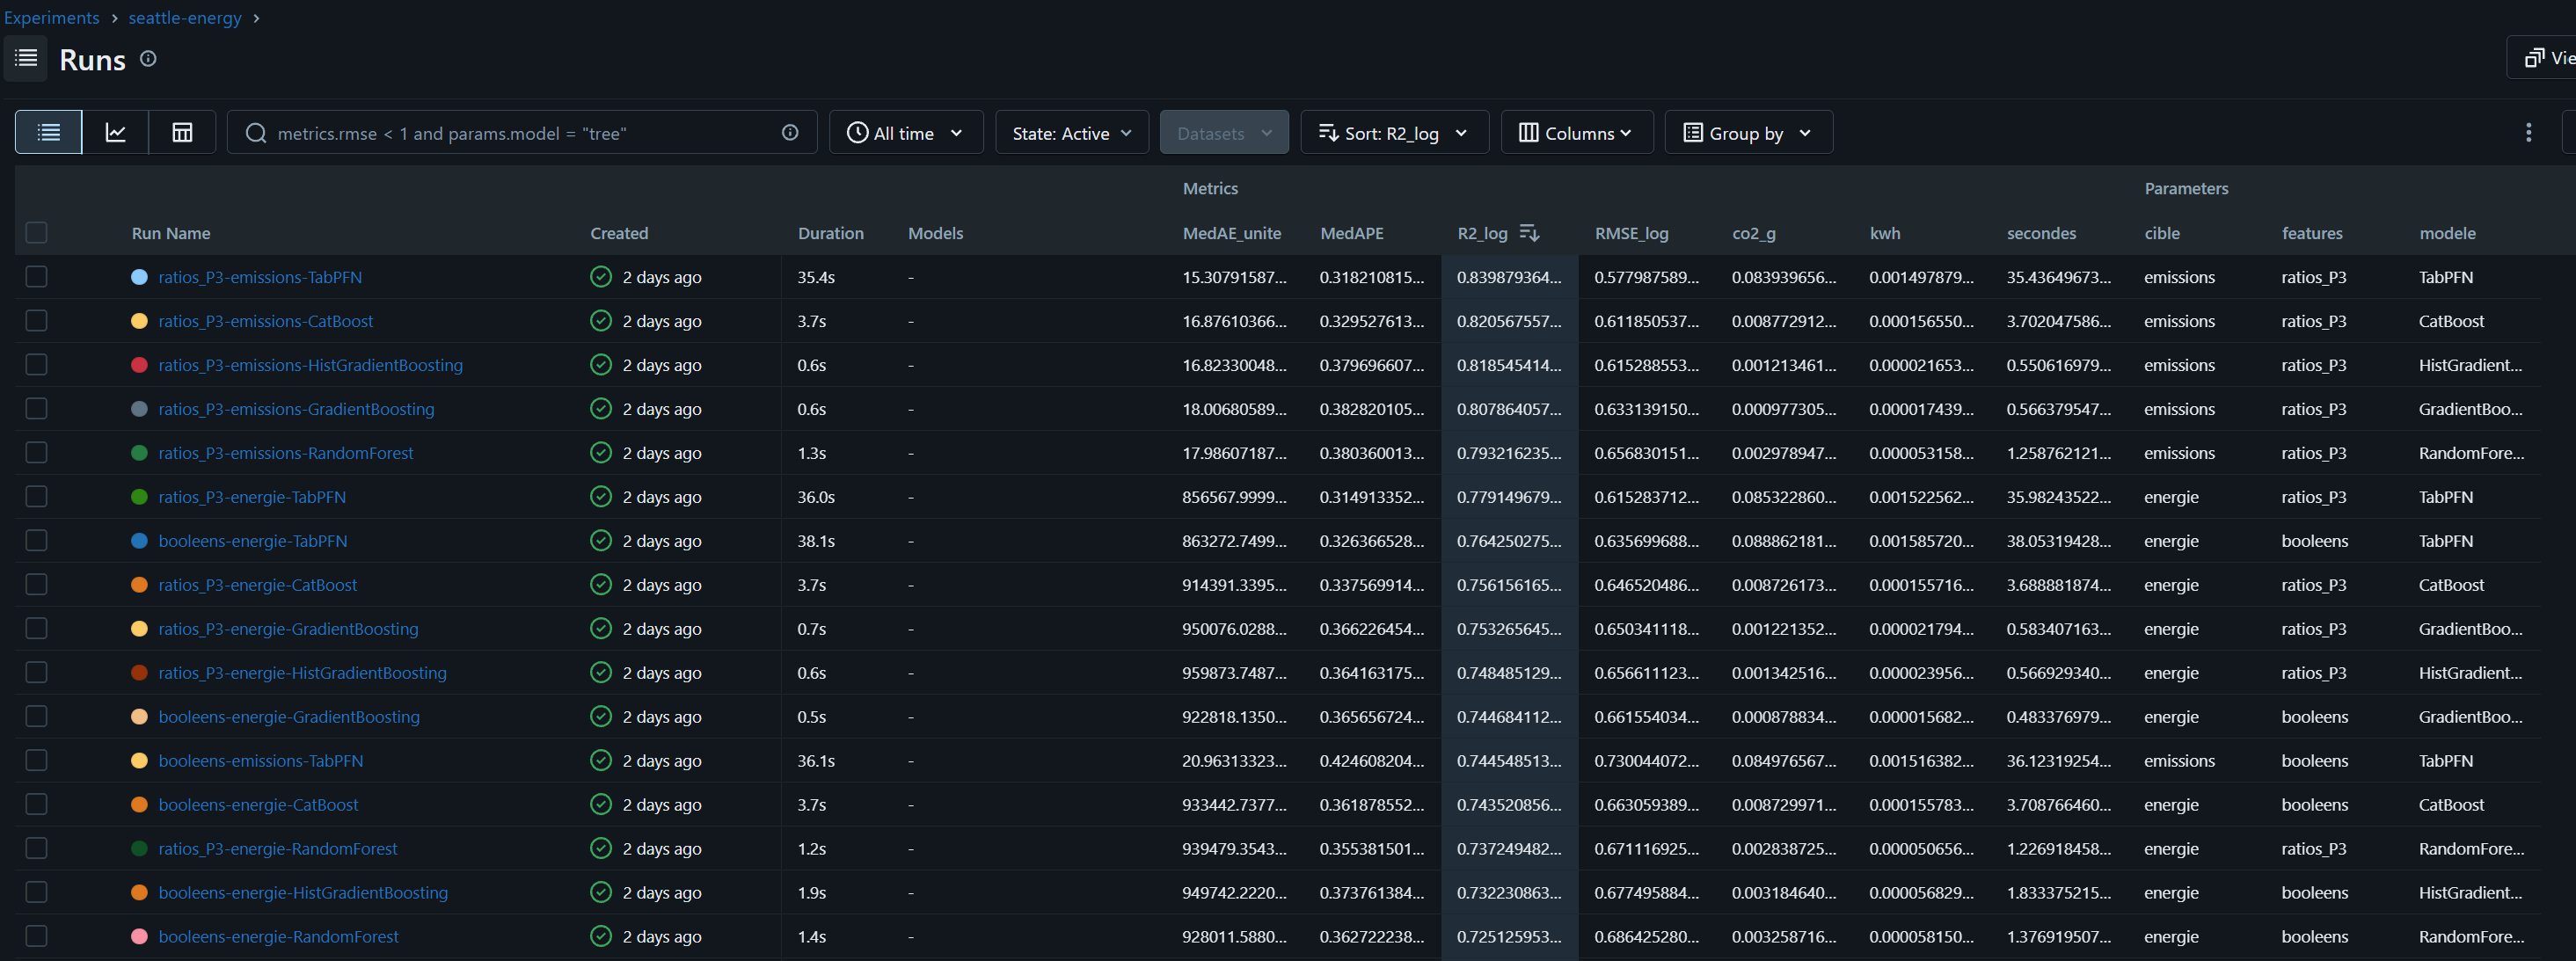
\includegraphics[width=\linewidth]{figures/mlflow-runs.png}
\caption{Registre d'expérimentations. Chaque exécution porte ses métriques, sa
durée et son empreinte, ce qui rend la comparaison « avec ratios / sans ratios »
vérifiable plutôt qu'affirmée.}
\end{figure}

\subsubsection*{Intégration et déploiement continus}

\begin{table}[H]
\centering
\small
\begin{tabularx}{\linewidth}{@{}L{3.6cm}X@{}}
\toprule
\textbf{Étape} & \textbf{Rôle} \\
\midrule
Analyse statique & Style et erreurs détectables sans exécution \\
Suite de tests & 61 tests : préparation, invariants du modèle, interface, configuration de déploiement \\
Déploiement conditionnel & Uniquement sur la branche principale, uniquement si tout est vert \\
\bottomrule
\end{tabularx}
\caption{Chaîne d'intégration et de déploiement.}
\end{table}

Un choix mérite d'être signalé : la chaîne installe les dépendances \textbf{depuis le
fichier de dépendances de l'application}, et non depuis l'environnement de
développement. La suite valide donc les artefacts contre la pile exacte que le
service fera tourner, et non contre celle du poste du développeur.


\begin{figure}[ht]
\centering
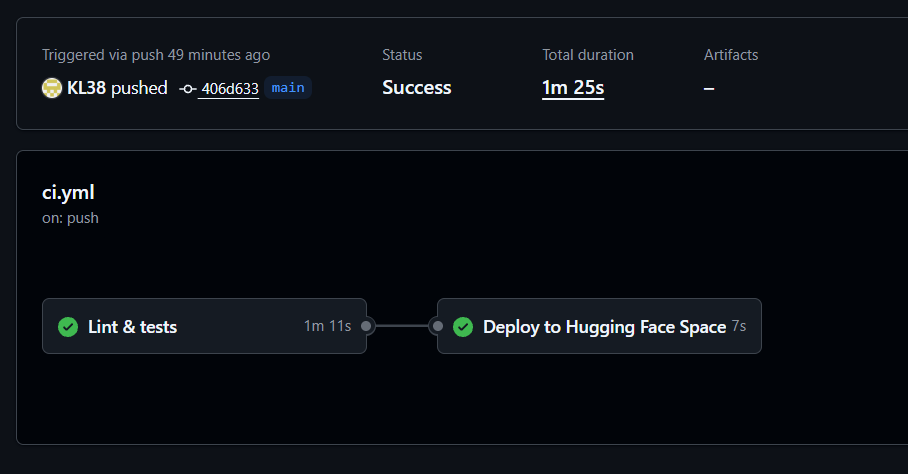
\includegraphics[width=0.78\linewidth]{figures/cicd-jobs.png}
\caption{Un cycle complet : les tests conditionnent le déploiement, qui ne
s'exécute que sur la branche principale.}
\end{figure}

\begin{figure}[ht]
\centering
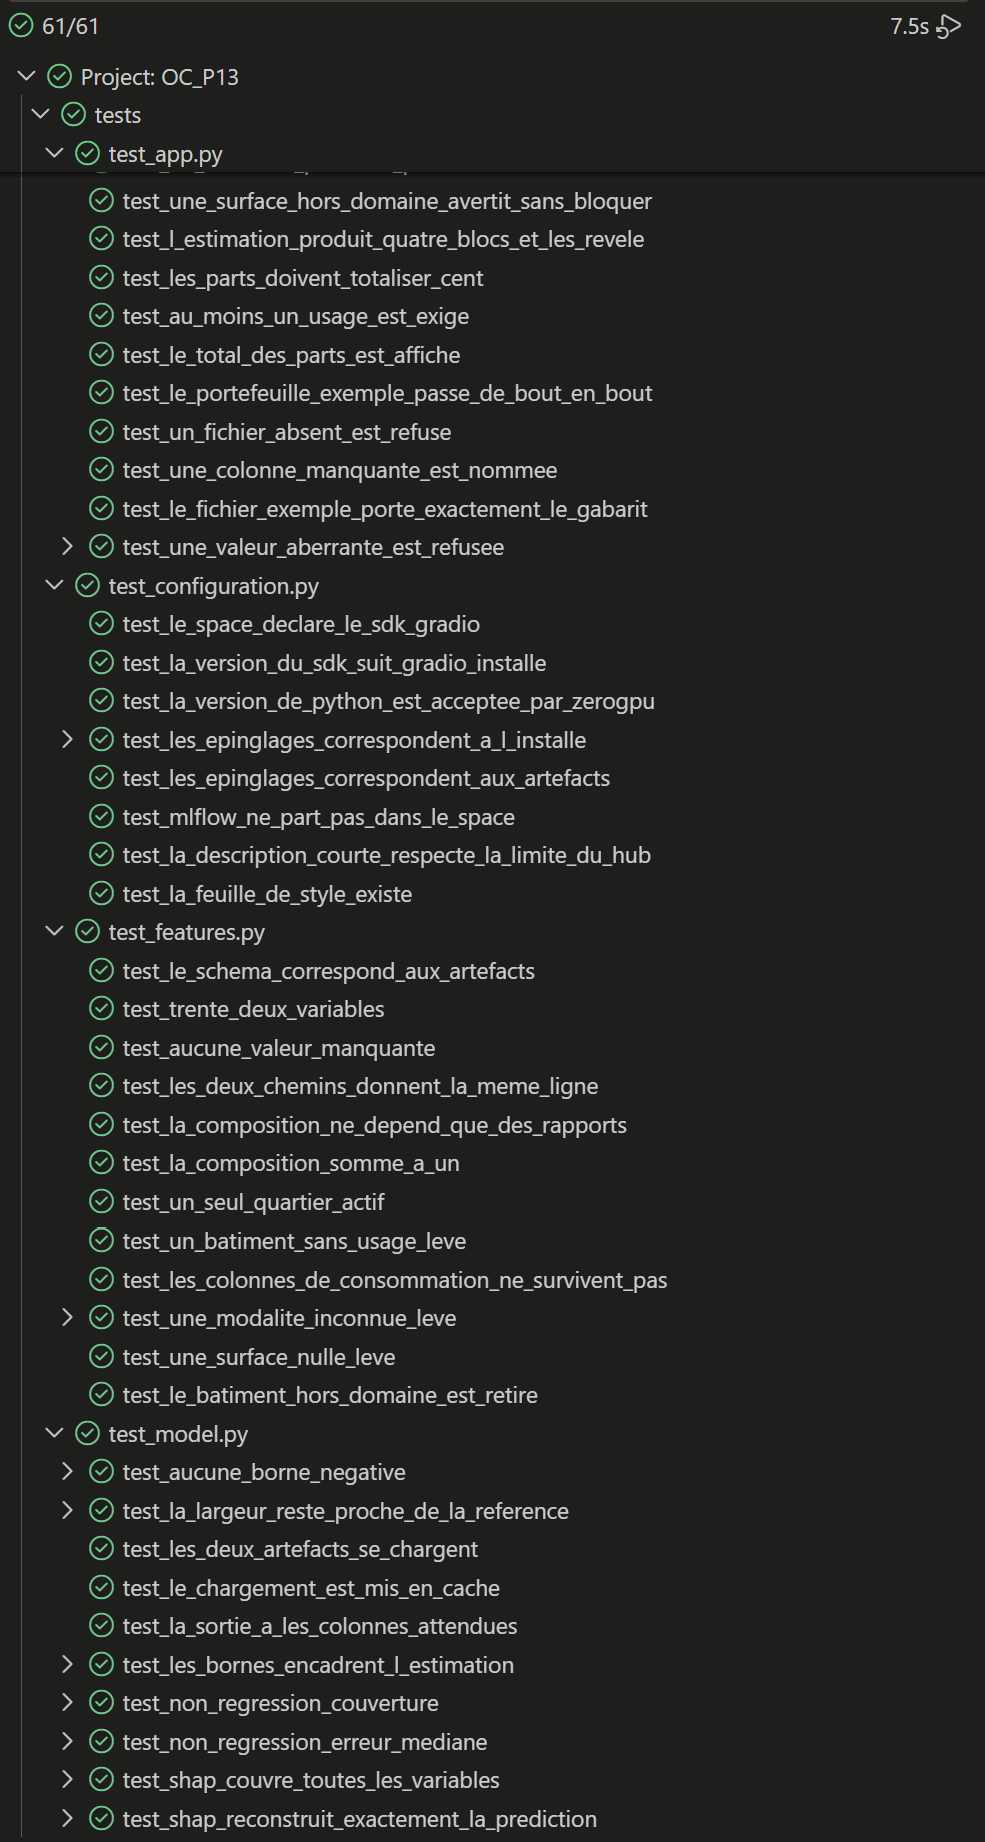
\includegraphics[height=13.5cm]{figures/tests-suite.png}
\caption{La suite de tests. Les quatre fichiers couvrent la préparation des
données, les invariants du modèle, les points d'entrée de l'interface et la
configuration de déploiement.}
\end{figure}

\subsubsection*{Trois défauts réels attrapés par le dispositif}

Le dispositif de contrôle n'est pas décoratif : il a produit trois constats que
la relecture humaine n'avait pas produits.

\begin{enumerate}[leftmargin=1.6em,itemsep=0.45em]
  \item \textbf{Une borne négative en production.} Un bâtiment sur \num{1655}
        sortait avec une borne basse d'émissions à $-0{,}134$~tCO\textsubscript{2}e.
        La cause est structurelle : la cible étant transformée en logarithme, la
        soustraction du quantile de conformité passe sous zéro pour une valeur
        minuscule. Corrigé par une projection sur le domaine physiquement
        admissible, sans perte de couverture.
  \item \textbf{Une dérive d'environnement.} L'exécution des tests depuis un
        environnement Python différent a révélé une bibliothèque d'apprentissage
        en version~1.8 alors que les artefacts avaient été produits en~1.9.
        Servi ainsi, le modèle aurait été désérialisé par une version autre que
        celle qui l'a ajusté — sans erreur ni avertissement. C'est le mode de
        panne silencieux que le test de configuration a été écrit pour attraper.
  \item \textbf{Une contrainte de plateforme non documentée.} Le déploiement a
        échoué sur une limite de longueur d'un champ de métadonnées, refusée non
        pas au niveau du champ mais de \emph{tout l'envoi}, après que les tests
        soient passés au vert. Un test vérifie désormais cette contrainte en
        amont.
\end{enumerate}

\subsubsection{Empreinte carbone : une mesure qui a tranché}
\label{sec:carbone}

L'empreinte de chaque entraînement a été mesurée modèle par modèle. Le résultat
utile n'est pas le total, il est dans les rapports.

\begin{table}[H]
\centering
\small
\begin{tabular}{@{}lrrr@{}}
\toprule
\textbf{Modèle} & \textbf{Durée} & \textbf{Énergie} & \textbf{$R^2$ énergie} \\
\midrule
GradientBoosting & 0,48~s & \textbf{0,016~Wh} & 0,745 \\
RandomForest & 1,38~s & 0,058~Wh & 0,725 \\
CatBoost & 3,71~s & 0,156~Wh & 0,744 \\
TabPFN & 38,05~s & \textbf{1,586~Wh} & 0,764 \\
\bottomrule
\end{tabular}
\caption{Consommation par modèle, cible énergie.}
\end{table}

\begin{constat}{Le seul arbitrage que la mesure a réellement tranché}
TabPFN consomme à lui seul \textbf{84\,\%} de l'énergie du banc d'essai complet,
soit \textbf{101 fois} le modèle retenu, pour un gain de deux points dans le bruit
d'échantillonnage. Il était déjà écarté pour sa licence ; la mesure lui donne un
\textbf{second motif de rejet, indépendant du premier}.
\end{constat}


\begin{figure}[ht]
\centering
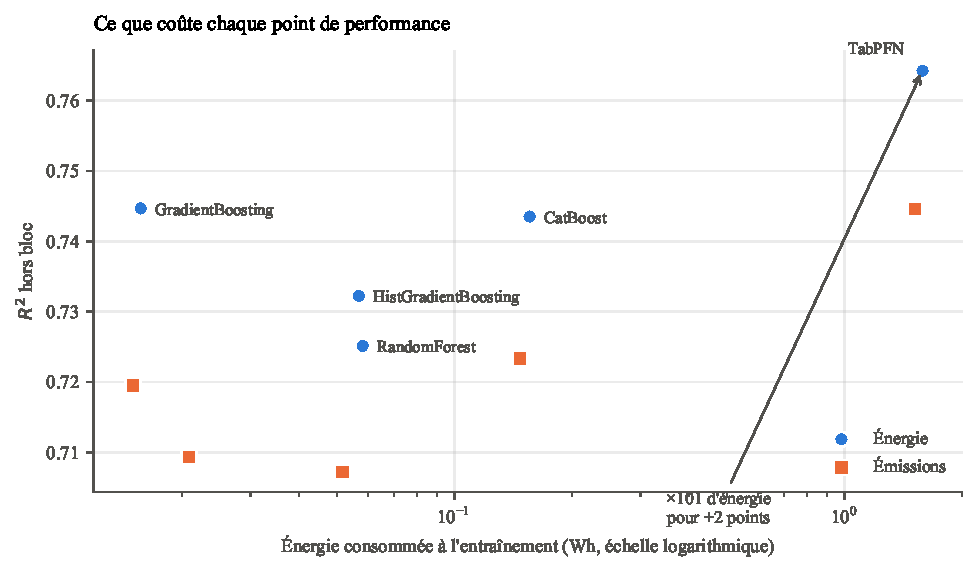
\includegraphics[width=\linewidth]{figures/empreinte-performance.pdf}
\caption{Coût énergétique de chaque point de performance. L'échelle des abscisses
est logarithmique : les cinq premiers modèles tiennent dans une décade, TabPFN
seul en occupe deux de plus.}
\end{figure}

Trois limites de l'indicateur sont documentées plutôt que passées sous silence :

\begin{itemize}[leftmargin=1.4em,itemsep=0.2em]
  \item \textbf{En absolu, la mesure n'arbitre rien.} Le banc d'essai complet a
        consommé 7,3~Wh et émis 0,41~g de CO\textsubscript{2}e — l'équivalent
        d'une ampoule LED allumée trois quarts d'heure.
  \item \textbf{Sous deux secondes, elle n'est pas reproductible.} Entre deux
        campagnes, les modèles les plus rapides varient de $+39\,\%$ et
        $-58\,\%$, quand les plus longs tiennent à quelques pourcents près.
  \item \textbf{Le lieu pèse plus que le modèle.} Le facteur de conversion mesuré
        est de 56~g\,CO\textsubscript{2}/kWh (mix français) ; sur un mix
        nord-américain le même calcul émettrait cinq à sept fois plus. Un chiffre
        d'empreinte n'est comparable qu'à un autre produit sur la même
        infrastructure.
\end{itemize}

\subsubsection{Le dispositif volontairement non implémenté}
\label{sec:monitoring}

Aucune supervision de dérive n'a été mise en place, et c'est une décision, pas un
oubli. Les données sont publiées une fois par an, le modèle est réentraîné au
même rythme, et le service compte un seul utilisateur métier sans équipe
d'exploitation. Une brique de supervision aurait ajouté un service à héberger, à
authentifier et à maintenir, pour détecter une dérive dont la fréquence
d'apparition est celle du réentraînement lui-même.

\begin{constat}{Ce que coûte une bonne pratique appliquée sans discernement}
Le coût de maintenance aurait dépassé le bénéfice attendu. L'arbitrage est
documenté ici précisément parce qu'un lecteur pourrait y voir une lacune : c'est
l'absence de justification, et non l'absence de l'outil, qui constituerait le
défaut.
\end{constat}

\newpage
